\documentclass[a4paper,14pt]{extarticle}

% Путь до папки с общими шаблонами
\newcommand{\pathToCommonFolder}{/home/denilai/Documents/repos/latex/Common}
% Название работы в титуле
\newcommand{\workname}{Отчет по лабораторной работе №2}
% Название дисциплины в титуле
\newcommand{\discipline}{Проектирование и разработка систем на базе ПЛИС}
% Название кафедры в титуле
\newcommand{\kafedra}{Кафедра Вычислительной техники}
% Тема работы в титуле
\newcommand{\theme}{Проектирование синтезируемой модели конечного автомата
	и её верификация средствами САПР Xilinx ISE 14.х.}
% Должность преподавателя в титуле
\newcommand{\rang}{ассистент}

% ФИО студента в титуле
\newcommand{\studentfio}{К.~Ю.~Денисов}
% ФИО преподавателя в титуле
\newcommand{\teacherfio}{А.~С.~Боронников}


\usepackage{tabularx}


\usepackage{booktabs}
\newcolumntype{b}{X}
\newcolumntype{s}{>{\hsize=.5\hsize}X}
\newcommand{\heading}[1]{\multicolumn{1}{c}{#1}}

% установка размера шрифта для всего документа
%\fontsize{20pt}{18pt}\selectfont
\usepackage{extsizes} % Возможность сделать 14-й шрифт

% Вставка заготовки преамбулы
% Этот шаблон документа разработан в 2014 году
% Данилом Фёдоровых (danil@fedorovykh.ru) 
% для использования в курсе 
% <<Документы и презентации в \LaTeX>>, записанном НИУ ВШЭ
% для Coursera.org: http://coursera.org/course/latex .
% Исходная версия шаблона --- 
% https://www.writelatex.com/coursera/latex/5.3

% В этом документе преамбула

% Для корректного использования русских символов в формулах
% пакеты hyperref и настройки, связанные с ним, стоит загуржать
% перед загрузкой пакета mathtext



% поддержка русских букв
% кодировка шрифта
%\usepackage[T2A]{fontenc} 
\usepackage{pscyr}

% использование ненумеровонного абзаца с добавлением его в содержаниеl

\newcommand{\anonsection}[1]{\section*{#1}\addcontentsline{toc}{section}{#1}}
\newcommand{\sectionunderl}[1]{\section*{\underline{#1}}}


% настройка окружения enumerate
\usepackage{enumitem}
\setlist{noitemsep}
\setlist[enumerate]{labelsep=*, leftmargin=1.5pc}

\usepackage{hyperref}

% сначала ставить \usepackage{extsizes} % Возможность сделать 14-й шрифт
% для корректной установки полей вставлять преамбулу следует в последнюю очередь (но перед дерективой замены \rmdefault)
\usepackage[top=20mm,bottom=25mm,left=35mm,right=20mm]{geometry} % Простой способ задавать поля

\hypersetup{				% Гиперссылки
	unicode=true,           % русские буквы в раздела PDF
	pdftitle={Заголовок},   % Заголовок
	pdfauthor={Автор},      % Автор
	pdfsubject={Тема},      % Тема
	pdfcreator={Создатель}, % Создатель
	pdfproducer={Производитель}, % Производитель
	pdfkeywords={keyword1} {key2} {key3}, % Ключевые слова
	colorlinks=true,       	% false: ссылки в рамках; true: цветные ссылки
	linkcolor=red,          % внутренние ссылки
	citecolor=black,        % на библиографию
	filecolor=magenta,      % на файлы
	urlcolor=blue           % на URL
}

%%% Работа с русским языком
\usepackage{cmap}					% поиск в PDF
\usepackage{mathtext} 				% русские буквы в формулах
\usepackage[T2A]{fontenc}			% кодировка
\usepackage[utf8]{inputenc}			% кодировка исходного текста
\usepackage[english,russian]{babel}	% локализация и переносы
\usepackage{indentfirst}
\frenchspacing

%для изменения названия списка иллюстраций
\usepackage{tocloft}


\renewcommand{\epsilon}{\ensuremath{\varepsilon}}
\renewcommand{\phi}{\ensuremath{\varphi}}
\renewcommand{\kappa}{\ensuremath{\varkappa}}
\renewcommand{\le}{\ensuremath{\leqslant}}
\renewcommand{\leq}{\ensuremath{\leqslant}}
\renewcommand{\ge}{\ensuremath{\geqslant}}
\renewcommand{\geq}{\ensuremath{\geqslant}}
\renewcommand{\emptyset}{\varnothing}

% Изменения параметров списка иллюстраций
\renewcommand{\cftfigfont}{Рисунок } % добавляем везде "Рисунок" перед номером
\addto\captionsrussian{\renewcommand\listfigurename{Список иллюстративного материала}}

\newcommand{\tm}{\texttrademark\ }
\newcommand{\reg}{\textregistered\ }


%%% Дополнительная работа с математикой
\usepackage{amsmath,amsfonts,amssymb,amsthm,mathtools} % AMS
\usepackage{icomma} % "Умная" запятая: $0,2$ --- число, $0, 2$ --- перечисление

%% Номера формул
%\mathtoolsset{showonlyrefs=true} % Показывать номера только у тех формул, на которые есть \eqref{} в тексте.
%\usepackage{leqno} % Нумереация формул слева

%% Свои команды
\DeclareMathOperator{\sgn}{\mathop{sgn}}

%% Перенос знаков в формулах (по Львовскому)
\newcommand*{\hm}[1]{#1\nobreak\discretionary{}
{\hbox{$\mathsurround=0pt #1$}}{}}


% отступ для первого абзаца главы или параграфа
%\usepackage{indentfirst}

%%% Работа с картинками
\usepackage{graphicx}  % Для вставки рисунков
\graphicspath{{images/}{screnshots/}}  % папки с картинками
\DeclareGraphicsExtensions{.pdf,.png,.jpg}
\setlength\fboxsep{3pt} % Отступ рамки \fbox{} от рисунка
\setlength\fboxrule{1pt} % Толщина линий рамки \fbox{}
\usepackage{wrapfig} % Обтекание рисунков текстом

%%% Работа с таблицами
\usepackage{array,tabularx,tabulary,booktabs} % Дополнительная работа с таблицами
\usepackage{longtable}  % Длинные таблицы
\usepackage{multirow} % Слияние строк в таблице

%%% Теоремы
\theoremstyle{plain} % Это стиль по умолчанию, его можно не переопределять.
\newtheorem{theorem}{Теорема}[section]
\newtheorem{proposition}[theorem]{Утверждение}

\theoremstyle{plain} % Это стиль по умолчанию, его можно не переопределять.
\newtheorem{work}{Практическая работа}[part]


 
 
\theoremstyle{definition} % "Определение"
\newtheorem{corollary}{Следствие}[theorem]
\newtheorem{problem}{Задача}[section]
 
\theoremstyle{remark} % "Примечание"
\newtheorem*{nonum}{Решение}



%%% Программирование
\usepackage{etoolbox} % логические операторы

%%% Страница

%	\usepackage{fancyhdr} % Колонтитулы
% 	\pagestyle{fancy}
%   \renewcommand{\headrulewidth}{0pt}  % Толщина линейки, отчеркивающей верхний колонтитул
% 	\lfoot{Нижний левый}
% 	\rfoot{Нижний правый}
% 	\rhead{Верхний правый}
% 	\chead{Верхний в центре}
% 	\lhead{Верхний левый}
%	\cfoot{Нижний в центре} % По умолчанию здесь номер страницы

\usepackage{setspace} % Интерлиньяж
\onehalfspacing % Интерлиньяж 1.5
%\doublespacing % Интерлиньяж 2
%\singlespacing % Интерлиньяж 1

\usepackage{lastpage} % Узнать, сколько всего страниц в документе.

\usepackage{soul} % Модификаторы начертания


\usepackage[usenames,dvipsnames,svgnames,table,rgb]{xcolor}


\usepackage{csquotes} % Еще инструменты для ссылок

%\usepackage[style=authoryear,maxcitenames=2,backend=biber,sorting=nty]{biblatex}

\usepackage{multicol} % Несколько колонок

\usepackage{tikz} % Работа с графикой
\usepackage{pgfplots}
\usepackage{pgfplotstable}

% модуль для вставки рыбы
\usepackage{blindtext}

\usepackage{listings}
\usepackage{color}


% для поворота отдельной страницы. Использовать окружение \landscape
\usepackage{pdflscape} 
\usepackage{rotating} 


\definecolor{mygreen}{rgb}{0,0.6,0}
\definecolor{mygray}{rgb}{0.5,0.5,0.5}
\definecolor{mymauve}{rgb}{0.58,0,0.82}


% пример импорта файла
%\lstinputlisting{/home/denilai/repomy/conf/distributions}

\lstset{
	language=Python,
	basicstyle=\footnotesize,        % the size of the fonts that are used for the code
	numbers=left,                    % where to put the line-numbers; possible values are (none, left, right)
	numbersep=5pt,                   % how far the line-numbers are from the code
	numberstyle=\tiny\color{mygray}, % the style that is used for the line-numbers
	stepnumber=2,                    % the step between two line-numbers. If it's 1, each line will be numbered
	% Tab - 2 пробела
	tabsize=2,    
	% Автоматический перенос строк
	breaklines=true,
	frame=single,
	breakatwhitespace=true,
	title=\lstname 
}



\author{Кирилл Денисов}
\title{Лабораторная работа №2}
\date{\today}

%если не нужна тема работы в отчете, то указать в скобках что-либо, иначе оаставить пустым
\renewcommand{\withouttheme}{}
%если нужна дата представления отчета, то указать в скобках что-либо
%\renewcommand{\withoutsubmissiondate}{1}

% установка полуторного интервала
% \usepackage{setspace}  
% \onehalfspacing

% использовать Times New Roman
\renewcommand{\rmdefault}{ftm}


\begin{document}
	\thispagestyle{empty}
	% Вставка первого титульного листа
	%\newcounter{withouttheme}

%\setcounter{withouttheme}{<n>} установить значение счетчика  withouttheme для определения, нужна ли тема
%    {0} - нужна
%    {1} - не нужна

%\setcounter{withoutsubmissiondate}{<n>} установить значение счетчика  withoutsubmissiondate для определения, нужна ли дата представления к защите
%     {0} - нужна
%     {1} - не нужена
\begin{center}
	\begin{figure}[h!]
		\begin{center}
		%\vspace{-10ex}
		
\includegraphics[width=0.17\linewidth]{\pathToCommonFolder/gerb}
		%\caption{}\label{pic:first}
		%	\vspace{5ex}
		\end{center}	
	\end{figure}
 	\small	МИНОБРНАУКИ РОССИИ \\
	Федеральное государственное бюджетное образовательное учреждение\\
						высшего образования\\
\normalsize					
\textbf{«МИРЭА – Российский технологический университет»\\
						РТУ МИРЭА}\\
						\noindent\rule{1\linewidth}{1pt}\\
       Институт информационных технологий\\ %\vspace{2ex}
					\kafedra\\
		\vspace{3ex}
			\large \textbf{\workname}  \\
		%\vspace{1ex}
						по дисциплине\\ «\discipline» \\
		\vspace{3ex}
		\ifnum \value{withouttheme}=0 {
			\textbf{Тема работы:}\\ <<\theme>>
		}
		\else {}
		\fi
\vspace{10ex}
\small
\begin{table}[h!]
\begin{tabular}{lp{0.6\linewidth}l}
	\textbf{Выполнил:} & студент группы ИВБО-02-19 & \\ 
	& & \studentfio \\%Д.~Н.~Федосеев\\%А.~М.~Сосунов\\%К.~Ю.~Денисов\\%И.~А.~Кремнев
	\textbf{Принял:} & \rang & \\
	& & \teacherfio \hfill\\
\end{tabular}
\end{table}
\end{center}
\ifnum \value{withoutsubmissiondate}=0 {
	\begin{flushleft}
		Работа представлена к защите <<\rule{3ex}{1pt}>>\rule{10ex}{1pt} 202\rule{1ex}{1pt} г.\hfill
	\end{flushleft}
\else {}
\fi

\normalsize
\begin{center}	
\vfill
Москва 2022
\end{center}

	\newpage
	\tableofcontents
	\newpage
	%\listoftables
\section{Ход работы}	
\subsection {Постановка задачи}
Требуется описать конечный автомат, представляющий собой генератор
фиксированной последовательности логических сигналов, в виде синтезируемой модели
на языке Verilog HDL.

Автомат должен иметь интерфейс, представленный на рис \ref{fig:fsmexample}.

% TODO: \usepackage{graphicx} required
\begin{figure}[htpb]
	\centering
	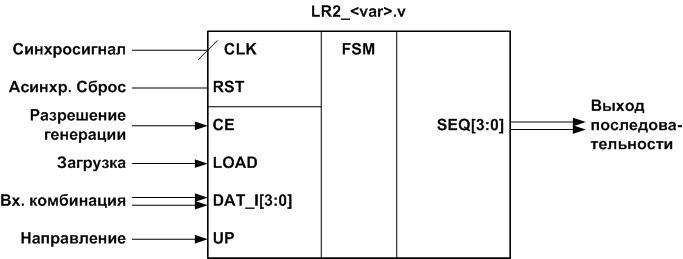
\includegraphics[width=0.5\linewidth]{images/fsm_example}
	\caption{Интерфейс цифрового автомата}
	\label{fig:fsmexample}
\end{figure}


Автомат является синхронным цифровым узлом, срабатывающим по восходящим
фронтам синхросигнала \textit{CLK}. Исключение составляет асинхронный вход сброса \textit{RST},
принудительно устанавливающий регистр автомата в исходное состояние (определяется
вариантом).
Автомат должен реагировать на входные воздействия согласно таблице \ref{tab:fsm state}.


\begin{table}[htbp]
		\begin{tabular}{|c|c|c|c|c|c|}
		\hline
		\textbf{RST}  & \textbf{CLK}  & \textbf{LOAD}  & \textbf{CE}  & \textbf{UP}  & \textbf{Действие} \\ \hline \hline
		1 & X  & X  & X  & X  & Асинхронный сброс SEQ <= Func(4'h0) \\ \hline
		0 & posedge & 1 & X  & X  & Загрузка SEQ <= Func(DAT\_I) \\ \hline
		0 & posedge & 0 & 1 & 0 & Обратная генерация SEQ <= Func(i-1) \\ \hline
		0 & posedge & 0 & 1 & 1 & Прямая генерация SEQ <= Func(i+1) \\ \hline
		0 & posedge & 0 &  & X  & Хранение SEQ <= SEQ \\ \hline
	\end{tabular}
	\caption{Таблица функционирования автомата}
	\label{tab:fsm state}
\end{table}


Последовательность генерируемых сигналов определяется функцией Func(i), где i --- 4-разрядный двоичный индекс, представляющий собой номер элемента
последовательности.

Инкремент индекса соответствует прямой генерации последовательности.
Декремент индекса соответствует обратной генерации последовательности.

Последовательность для каждого варианта выполнения работы определяется из
таблицы вариантов следующим образом: индекс \textit{i} задан входными комбинациями от \textit{F} до
0 в верхней строке таблицы, а выходные комбинации \textit{Func(i)}, формируемые на выходах
\textit{SEQ[3:0]}, заданы строкой таблицы, соответствующей выбранному варианту.
Допускается использовать различные варианты кодировки состояний автомата.
Автомат может иметь организацию согласно абстрактным моделям Мили или Мура.

\subsection {Индивидуальный вариант 149}
Требуется описать конечный автомат, представляющий собой генератор
фиксированной последовательности логических сигналов, в виде синтезируемой модели
на языке Verilog HDL согласно данной таблице истинности и вектор-функции (см. таблицу \ref{tab:func-vector}).

\begin{table}[htbp]
	\begin{center}
	\begin{tabular}{|c|c|c|c|c|c|c|c|c|c|c|c|c|c|c|c|}
		\hline
		F & E & D & C & B & A & 9 & 8 & 7 & 6 & 5 & 4 & 3 & 2 & 1 & 0 \\ \hline\hline
		0 & 4 & 4 & 8 & 3 & 0 & 7 & 2 & 2 & D & 7 & C & 5 & 2 & A & C \\ \hline
	\end{tabular}
	\caption{Вектор-функция}
	\label{tab:func-vector}
\end{center}
\end{table}

\subsection{Структурная схема автомат}
Построим структурную схему цифрового устройства. Используем делитель частоты для снижения частоты тактового генератора, фильтр дребезга для использования кнопок в качестве устройств ввода. См. рис. \ref{fig:fsm-struct}.
% TODO: \usepackage{graphicx} required
\begin{figure}[htpb]
	\centering
	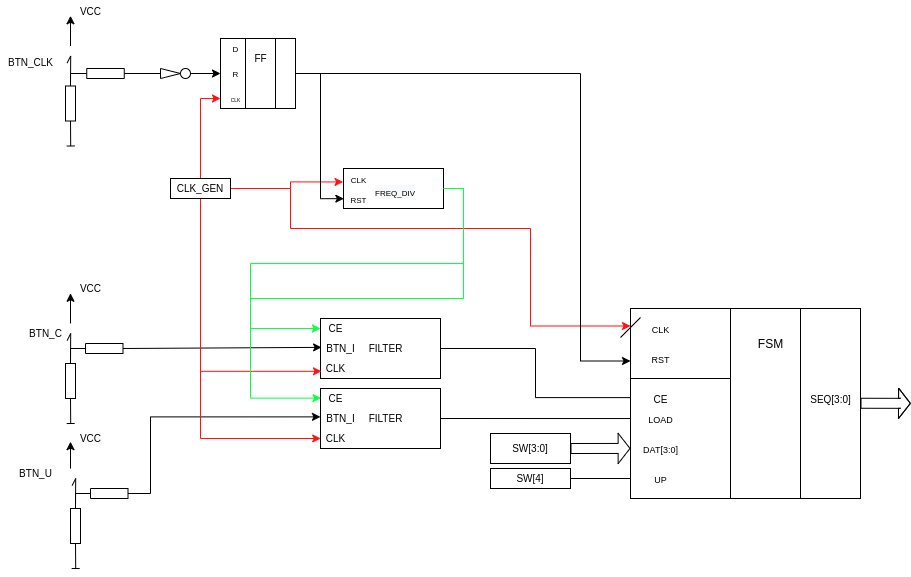
\includegraphics[width=0.7\linewidth]{images/fsm-struct}
	\caption{Структурная схема  устройства}
	\label{fig:fsm-struct}
\end{figure}


\subsection{Кодировка состояний автомата в двоичной и шестнадцатиричной системах}
Опишем модуль behaviour.v, указав в нем состояния автомата, приведенные в шестнадцатеричной системе.

\lstinputlisting{/home/denilai/Documents/repos/latex/scripts/behaviour.v}

\newpage
\subsection{Граф состояний}
Опишем граф перехода цифрового автомата согласно указанным режимам работы (переход в следующее или предыдущее состояние, загрузка состояния, хранение, сброс). См рис. \ref{fig:graph}.
% TODO: \usepackage{graphicx} required
\begin{figure}[htbp]
	\centering
	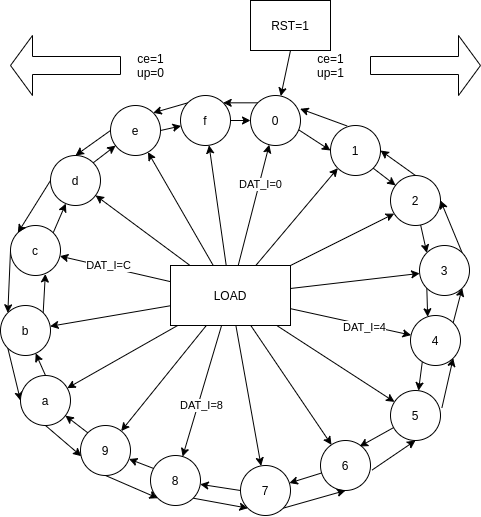
\includegraphics[width=0.4\linewidth]{images/graph}
	\caption{Граф переходов}
	\label{fig:graph}
\end{figure}

%\newpage
\subsection{Создание проекта САПР Xilinx ISE}
Приведем содержание verilog-модуля, описывающего цифровой автомат.
\lstinputlisting{/home/denilai/Documents/repos/latex/scripts/fsm.v}

Приведем содержание verilog-модуля, описывающего делитель частоты.
\lstinputlisting{/home/denilai/Documents/repos/latex/scripts/freq_div.v}
\newpage

Приведем содержание verilog-модуля, описывающего фильтр дребезга. \lstinputlisting{/home/denilai/Documents/repos/latex/scripts/m_btn_filter.v}

Приведем содержание verilog-модуля, описывающего тестовое окружение, описывающее входные воздействия для данной модели. \lstinputlisting{/home/denilai/Documents/repos/latex/scripts/test-fsm.v}

Приведем содержание verilog-модуля верхнего уровня 
\lstinputlisting{/home/denilai/Documents/repos/latex/scripts/top2.v}



\subsection{Тестирование и отладка средствами симулятора iSim}
После компоновки проекта, подключения модуля верхнего уровня, проведем верификацию спроектированных моделей с помощью симулятора iSim из состава САПР Xilinx ISE Design Suite. Результаты тестирования можно видеть на рис. \ref{fig:test-result1} и \ref{fig:test-result2}.

% TODO: \usepackage{graphicx} required
\begin{figure}[htpb]
	\centering
	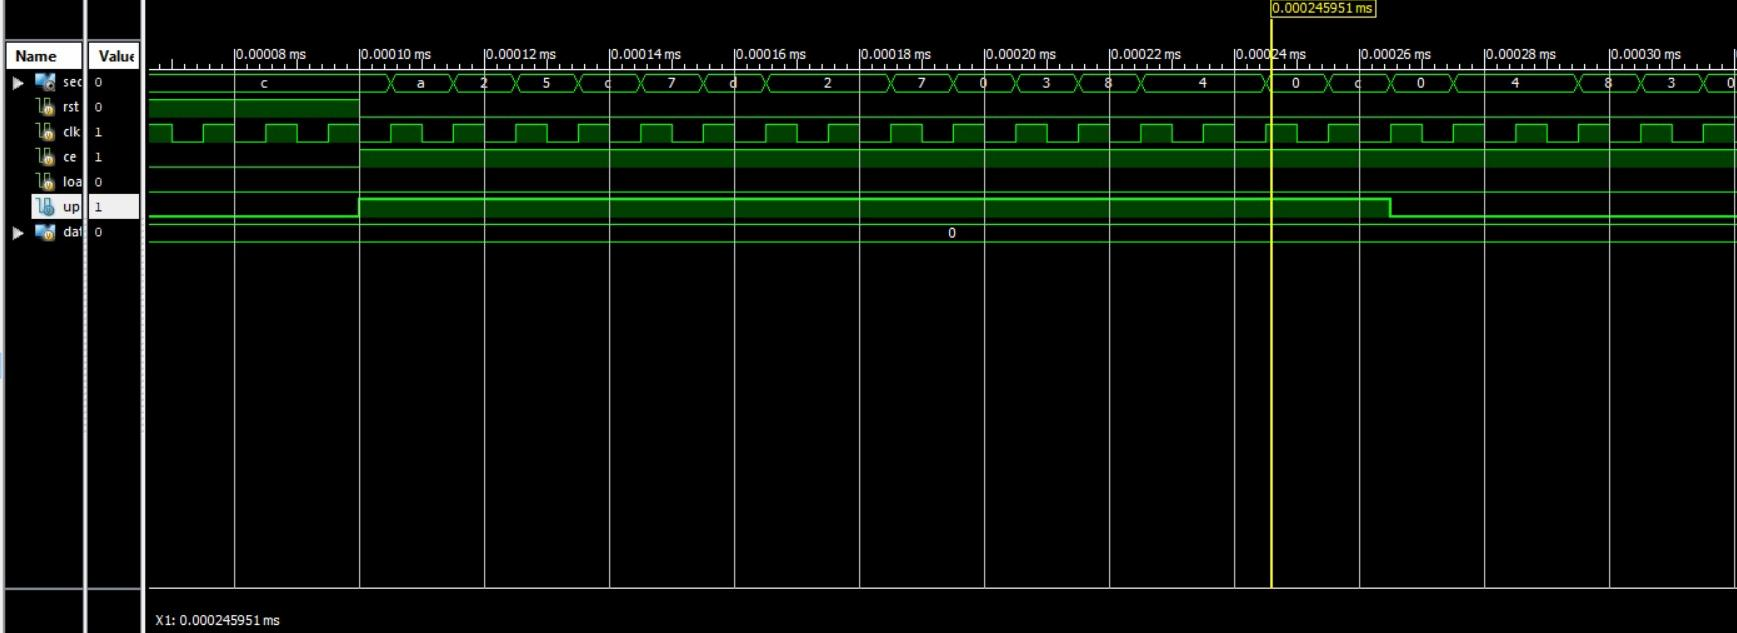
\includegraphics[width=\linewidth]{images/test-result2.1}
	\caption{Вывод iSim }
	\label{fig:test-result1}
\end{figure}

\begin{figure}[htpb]
	\centering
	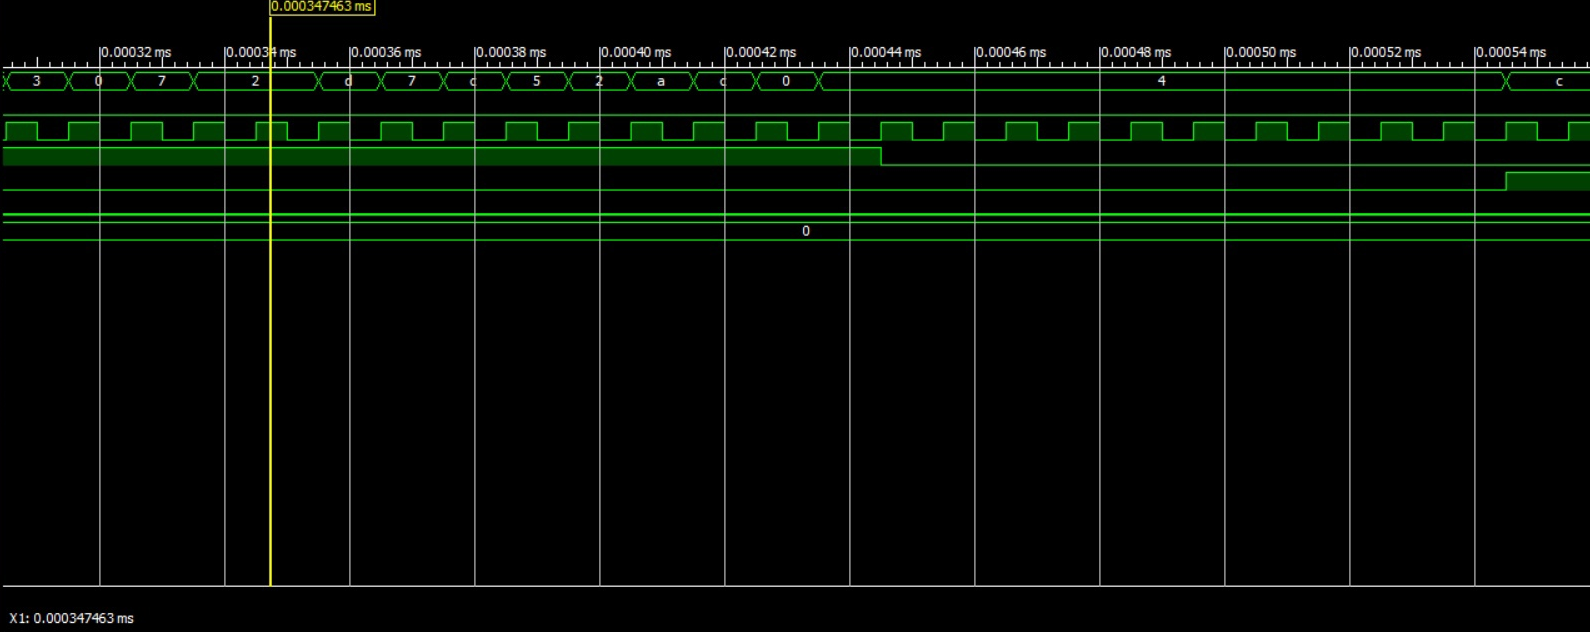
\includegraphics[width=\linewidth]{images/test-result2.3}
	\caption{Вывод iSim }
	\label{fig:test-result2}
\end{figure}
Приведем структуру проекта. См. рис. \ref{fig:file-tree}.
\begin{figure}[htpb]
	\centering
	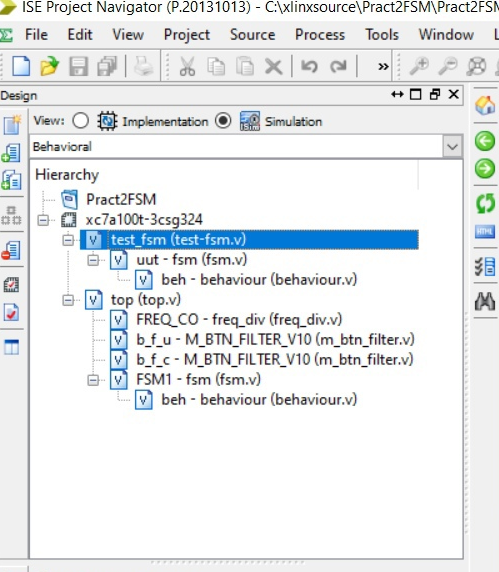
\includegraphics[width=0.4\linewidth]{images/file-tree}
	\caption{Иерархия проекта }
	\label{fig:file-tree}
\end{figure}

\newpage
\section{Вывод}
В ходе данной практической работы нами были получены общие навыки работы с программным обеспечением Xilinx ISE Design Suite, изучены основы языка Verilog.

С помощью полученных знаний был спроектирован конечный автомат, представляющий собой генератор
фиксированной последовательности логических сигналов, в виде синтезируемой модели.
\end{document}
